%Harj. Tehtävät Luku 2.1, vastausten tekijä Valtteri Vistiaho 9.11.2013
\begin{tehtava}
    Onko lause atomilause?
    \begin{alakohdat}
        \alakohta{Tampere on Pirkanmaalla.}
        \alakohta{Kajaani on Suomen pääkaupunki.}
        \alakohta{Hattu pois päästä!}
        \alakohta{On olemassa suurin alkuluku.}
        \alakohta{Onko avaruudessa elämää?}
        \alakohta{$5 + 12 = 18$.}
    \end{alakohdat}

    \begin{vastaus}
        \begin{alakohdat}
            \alakohta{On}
            \alakohta{On}
            \alakohta{Ei}
            \alakohta{On}
            \alakohta{Ei, ?????????} %En ole täysin varma vastauksesta
            \alakohta{On, ?????????} %En ole täysin varma vastauksesta
        \end{alakohdat}
    \end{vastaus}
    
\end{tehtava}

\begin{tehtava}
    Kirjoita lauseen negaatio.
    \begin{alakohdat}
        \alakohta{Tänään on maanantai.}
        \alakohta{$2+3=5$.}
        \alakohta{Luku on negatiivinen.}
        \alakohta{Ainakin yhdellä ryhmämme opiskelijalla on ruskeat silmät.}
        \alakohta{Kymmenessä sivussa tekstiä on vähintään seitsemän virhettä.}
        \alakohta{Kesä Välimerellä on kuuma ja aurinkoinen.}
    \end{alakohdat}

    \begin{vastaus}
        \begin{alakohdat}
            \alakohta{Tänään ei ole maanantai.}
            \alakohta{$2+3\neq5$}
            \alakohta{Luku on positiivinen.}
            \alakohta{Ainakin yhdellä ryhmämme opiskelijalla ei ole ruskeita silmiä.}
            \alakohta{Kymmenessä sivussa tekstiä on vähintään seitsemän virhettä.}
            \alakohta{Kesä Välimerellä on kylmä ja pilvinen.}
        \end{alakohdat}
    \end{vastaus}
    
\end{tehtava}

\begin{tehtava}
    Olkoot lause $A$: ''veikkasin lottorivin'' ja lause $B$: ''voitin miljoona euroa''. Kirjoita suomen kielellä lauseet
    \begin{alakohdat}
        \alakohta{$\lnot A$,}
        \alakohta{$A\lor B$,}
        \alakohta{$A\land B$,}
        \alakohta{$A\land \lnot B$,}
        \alakohta{$\lnot A\lor (A\land B)$,}
        \alakohta{$\lnot A\land \lnot B$.}
    \end{alakohdat}

    \begin{vastaus}
        \begin{alakohdat}
            \alakohta{En veikannut lottoriviä.}
            \alakohta{Veikkasin lottorivin tai voitin miljoona euroa.}
            \alakohta{Veikkasin lottorivin ja voitin miljoona euroa.}
            \alakohta{Veikkasin lottorivin ja en voittanut miljoonaa euroa.}
            \alakohta{En veikannut lottoriviä tai veikkasin lottorivin ja voitin miljoona euroa.}
            \alakohta{En veikannut lottoriviä enkä voittanut miljoonaa euroa.}
        \end{alakohdat}
    \end{vastaus}
    
\end{tehtava}

\begin{tehtava}
    Olkoot lause $A$: ''on kaunis kesäpäivä'',  lause $B$: ''lokit kirkuvat'' ja lause $C$: ''kävelen rannalla''. Kirjoita suomen kielellä lauseet
    \begin{alakohdat}
        \alakohta{$\lnot A\lor B$,}
        \alakohta{$A\land B \land C$,}
        \alakohta{$\lnot(A\land C)$,}
        \alakohta{$(A\land C)\lor (B\land
\lnot C)$.}
    \end{alakohdat}

    \begin{vastaus}
        \begin{alakohdat}
            \alakohta{Ei ole kaunis kesäpäivä tai lokit kirkuvat.}
            \alakohta{On kaunis kesäpäivä, lokit kirkuvat ja kävelen rannalla.}
            \alakohta{Ei ole totta, että on kaunis kesäpäivä ja kävelen rannalla.}
            \alakohta{On kaunis kesäpäivä ja kävelen rannalla tai lokit kirkuvat ja en kävele rannalla.}
        \end{alakohdat}
    \end{vastaus}
    
\end{tehtava}

\begin{tehtava}
    Olkoot $A$: ''on pilvistä'' ja $B$: ''sataa
lunta''. Formalisoi seuraavat lauseet eli kirjoita ne
lauseiden $A$ ja $B$ sekä konnektiivien $\lnot$, $\land$
ja $\lor$ avulla.
    \begin{alakohdat}
        \alakohta{On pilvistä ja sataa lunta.}
        \alakohta{On pilvistä, mutta ei sada lunta.}
        \alakohta{Ei ole pilvistä eikä sada lunta.}
        \alakohta{On pilvistä tai sataa lunta.}
        \alakohta{On pilvistä ja sataa lunta tai ei ole pilvistä
eikä sada lunta.}
    \end{alakohdat}

    \begin{vastaus}
        \begin{alakohdat}
            \alakohta{$A\land B$}
            \alakohta{$A\land \lnot B$}
            \alakohta{$\lnot A \land \lnot B$}
            \alakohta{$A \lor B$}
            \alakohta{$(A\land B)\lor \lnot A\land \lnot B$}
        \end{alakohdat}
    \end{vastaus}
    
\end{tehtava}

\begin{tehtava}
    Formalisoi lauseet:
    \begin{alakohdat}
        \alakohta{Mustikat polun varrella ovat kypsiä tai
alueella ei ole nähty karhuja.}
        \alakohta{Ei ole totta, että mustikat polun varrella ovat
kypsiä tai alueella on nähty karhuja.}
        \alakohta{Mustikat polun varrella ovat kypsiä, mutta
alueella ei ole nähty karhuja, tai sitten mustikat eivät
ole kypsiä ja alueella on nähty karhuja.}
        \alakohta{Karhuja ei ole nähty alueella ja polulla
vaeltaminen on turvallista, mutta mustikat ovat kypsiä.}
    \end{alakohdat}

    \begin{vastaus}
    Olkoot $A$: ''Mustikat polun varrella ovat kypsiä.'', $B$: ''Alueella on nähty karhuja.'' ja $C$: ''Polulla vaeltaminen on turvallista.''
        \begin{alakohdat}
            \alakohta{$A \lor \lnot B$}
            \alakohta{$\lnot(A\lor B)$}
            \alakohta{$(A\land \lnot B)\lor(\lnot A\land B)$}
            \alakohta{$\lnot B\land C\land A)$}
        \end{alakohdat}
    \end{vastaus}
    
\end{tehtava}

\begin{tehtava}
    
    \begin{alakohdat}
        \alakohta{Laadi totuustaulu lauseelle $\lnot A\lor \lnot
B$. Millä atomilauseiden $A$ ja $B$ totuusarvoilla lause
on tosi?}
        \alakohta{Laadi totuustaulu lauseelle $\lnot(A\land B)$.
Millä atomilauseiden $A$ ja $B$ totuusarvoilla lause on
tosi? Vertaa a-kohdan tulokseen.}
        \alakohta{Keksi atomilauseet $A$ ja $B$ ja ilmaise a- ja
b-kohtien lauseet suomen kielellä.}
    \end{alakohdat}

    \begin{vastaus}
        \begin{alakohdat}
            \alakohta{
            \begin{center}
		    \begin{tabular}{|c|c|c|c|c|}\hline
		    $A$ & $B$ & $\lnot A$ & $\lnot B$ & $\lnot A\lor \lnot B$\\ \hline
		    $1$ & $1$ & $0$ & $0$ & $0$  \\ %\hline
		    $1$ & $0$ & $0$ & $1$ & $1$  \\
		    $0$ & $1$ & $1$ & $0$ & $1$  \\
		    $0$ & $0$ & $1$ & $1$ & $1$  \\ \hline
\end{tabular}
\end{center}}
            \alakohta{
            \begin{center}
		    \begin{tabular}{|c|c|c|}\hline
		    $A$ & $B$ & $\lnot(A\land B)$\\ \hline
		    $1$ & $1$ & $0$  \\ %\hline
		    $1$ & $0$ & $1$  \\
		    $0$ & $1$ & $1$  \\
		    $0$ & $0$ & $1$  \\ \hline
\end{tabular}
\end{center}}
            \alakohta{Ei sada tai ei tuule.\newline Ei ole totta, että sataa ja tuulee.}
        \end{alakohdat}
    \end{vastaus}
    
\end{tehtava}

\begin{tehtava}
    Laadi totuustaulu lauseelle $(A\land B)\lor \lnot (B\lor C)$.

    \begin{vastaus}
        \begin{center}
		    \begin{tabular}{|c|c|c|c|c|c|c|}\hline
		    $A$ & $B$ & $C$ & $B\lor C$ & $A\land B$ & $\lnot (B\lor C)$ & $(A\land B)\lor \lnot (B\lor C)$\\ \hline
		    $1$ & $1$ & $1$ & $1$ & $1$ & $0$ & $1$  \\ %\hline
		    $1$ & $1$ & $0$ & $1$ & $1$ & $0$ & $1$  \\
		    $1$ & $0$ & $1$ & $1$ & $0$ & $0$ & $0$  \\
		    $1$ & $0$ & $0$ & $0$ & $0$ & $1$ & $1$  \\
		    $0$ & $1$ & $1$ & $1$ & $0$ & $0$ & $0$  \\
		    $0$ & $1$ & $0$ & $1$ & $0$ & $0$ & $0$  \\
		    $0$ & $0$ & $1$ & $1$ & $0$ & $0$ & $0$  \\
		    $0$ & $0$ & $0$ & $0$ & $0$ & $1$ & $1$  \\ \hline
\end{tabular}
\end{center}
    \end{vastaus}
    
\end{tehtava}

\begin{tehtava}
    Olkoot atomilauseet $A$: ''$x < -1$'', $B$: ''$x > 1$''  ja $C$: ''$x = 1$''. Formalisoi  lauseet
    \begin{alakohdat}
        \alakohta{$x\neq 1$,}
        \alakohta{$x \ge 1$,}
        \alakohta{$x \ge -1$,}
        \alakohta{$x < 1$,}
        \alakohta{$-1 \le x \le  1$,}
        \alakohta{$x <  -1$ tai $x  \ge 1$.}
    \end{alakohdat}

    \begin{vastaus}
        \begin{alakohdat}
            \alakohta{$\lnot C$}
            \alakohta{$B\lor C$}
            \alakohta{$\lnot A$}
            \alakohta{$\lnot(B\lor C)$}
            \alakohta{$\lnot(A\land B$}
            \alakohta{$A\lor (B\lor C)$}
        \end{alakohdat}
    \end{vastaus}
    
\end{tehtava}

\begin{tehtava}
    Saarella asuu haltijoita ja menninkäisiä. Turisti tapasi kaksi saarelaista, Hipsun ja Vipsun. Hipsu sanoi: ''Hillat ovat kypsiä ja kalaonni on suotuisa, tai sitten hillat eivät ole kypsiä tai kalaonni ei ole suotuisa.'' Vipsu väitti: ''Hillat ovat kypsiä ja kalaonni on suotuisa, mutta hillat eivät ole kypsiä tai kalaonni ei ole suotuisa.'' Tutki totuustaulun avulla Hipsun ja Vipsun väitteiden totuusarvoja. Mitä voidaan päätellä totuustaulun avulla, kun tiedetään, että saaren asukkaista haltijat valehtelevat aina ja menninkäiset puhuvat aina totta? Saiko vierailija käyttökelpoista tietoa marjasadosta tai kalaonnesta?

    \begin{vastaus}
    Olkoot $A$: ''Hillat ovat kypsiä.'' ja $B$: ''Kalaonni on suotuisa.''
    \begin{center}
		    \begin{tabular}{|c|c|c|c|c|c|c|c|}\hline
		    $A$ & $B$ & $\lnot A$ & $\lnot B$ & $A\land B$ & 
		         $\lnot A\lor \lnot B$ & $(A \land B)\lor(\lnot A\lor \lnot B)$ & $(A\land B)\land(\lnot A\lor \lnot B)$ \\ \hline
		    $1$ & $1$ & $0$ & $0$ & $1$ & $0$ & $1$ & $0$  \\ %\hline
		    $1$ & $0$ & $0$ & $1$ & $0$ & $1$ & $1$ & $0$  \\
		    $0$ & $1$ & $1$ & $0$ & $0$ & $1$ & $1$ & $0$  \\
		    $0$ & $0$ & $1$ & $1$ & $0$ & $1$ & $1$ & $0$  \\ \hline
\end{tabular}
\end{center}
	??????????????????????????????????????????????????????????????? %Tehtävä on melko epäselvä, mahdollisesti monta eri tulkintaa.
    \end{vastaus}
    
\end{tehtava}

\begin{tehtava}
    Loogisilla piireillä suoritetaan digitaalisissa laitteissa erilaisia loogisia operaatioita. Loogisen piirin toimintaa voidaan kuvata esimerkiksi seuraavalla kaaviolla.

\medskip

\begin{center}
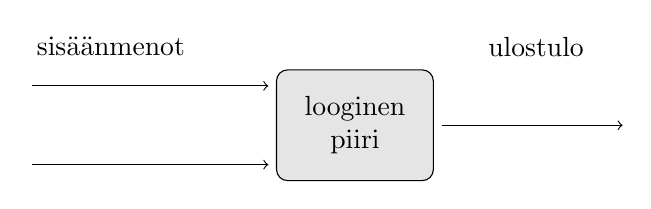
\begin{tikzpicture}
\node [rectangle, draw, fill=gray!20, text width=5em, text centered, rounded corners, minimum height=4em] at (4.1,1) {looginen piiri};
\draw [->] (0,0.5) -- (3,0.5);
\draw [->] (0,1.5) -- (3,1.5);
\draw [->] (5.2,1) -- (7.5,1);


\node at (1,2) {sisäänmenot};
\node at (6.4,2) {ulostulo};
\end{tikzpicture}
\end{center}

\medskip

Loogisella piirillä on yksi tai useampi sisäänmeno ja
yksi tai useampi ulostulo. Tämän kirjan esimerkeissä ja
tehtävissä käsitellään vain yhden ulostulon piirejä.
Sisäänmenojen ja ulostulon signaalin arvo
voi olla 1 tai 0. Edellisessä tapauksessa johtimessa on
jännite, jälkimmäisessä tapauksessa ei ole.

Loogiset piirit kootaan loogisista porteista. Seuraavassa
taulukossa on lueteltu loogiset portit, niiden toiminta
ja toimintaa vastaava looginen konnektiivi.

%\newpage

\small

\begin{center}
\begin{tabular}{|>{\centering}m{1.5cm}|>{\raggedright}m{3.8cm}|c|>{\centering\arraybackslash}m{2cm}|}
\hline
Looginen portti & \centering Toiminta & Piirrosmerkki & Looginen konnektiivi \\
% \begin{tabular}{c}
% %Toimintaa \\
% %	vastaava \\
% Looginen \\
% konnektiivi
% \end{tabular}
\hline

Tai &
Tai-portti antaa jännitteen, kun ainakin toisessa sisäänmenossa on jännite. &

%\begin{center}
\raisebox{-.5\height}{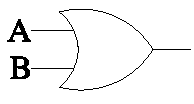
\includegraphics[width=2.5cm]{pictures/boole/or-ABC}}
%\end{center}
&
$A\lor B$
\\ \hline

Ja &
Ja-portti antaa jännitteen vain silloin, kun molemmissa sisäänmenoissa on jännite. &

%\begin{center}
\raisebox{-.5\height}{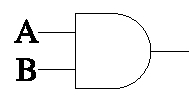
\includegraphics[width=2.5cm]{pictures/boole/and-ABC}}
%\end{center}
&
$A\land B$
\\ \hline

Ei &
Ei-portti antaa jännitteen silloin, kun sisäänmenossa ei ole jännitettä, ja kääntäen. &
%\begin{center}
\raisebox{-.5\height}{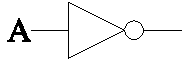
\includegraphics[width=2.5cm]{pictures/boole/not-ABC}}
%\end{center}
&
$\lnot A$
\\ \hline

\end{tabular}

\end{center}

\normalsize

%\newpage

\bigskip

Esimerkiksi looginen piiri

\medskip

\begin{center}
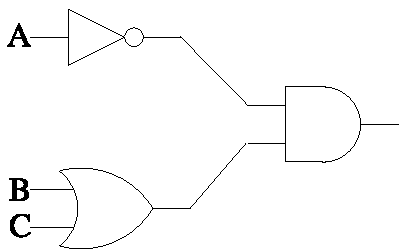
\includegraphics[width=3.5cm]{pictures/boole/boolesim-ABC}
\end{center}

\medskip
\noindent
koostuu kolmesta loogisesta portista ja vastaa
lausetta \mbox{$\lnot A\land (B \lor C)$}. %Muutettu alkuperäisestä, virhe joko tekstissä tai kuvassa.

%{\bf Tehtäviä}

%\begin{enumerate}
Muodosta seuraavia piirejä vastaavat lauseet.
    \begin{alakohdat}
        \alakohta{\begin{center}
		   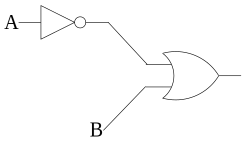
\includegraphics[width=3.5cm]{pictures/boole/boolt-a-ABC}
		   \end{center}}
	\alakohta{\begin{center}
		   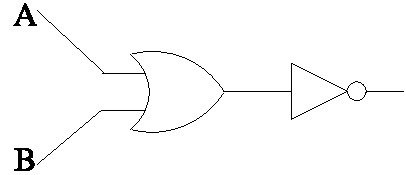
\includegraphics[width=3.5cm]{pictures/boole/boolt-b-ABC}
		   \end{center}}
        \alakohta{\begin{center}
		   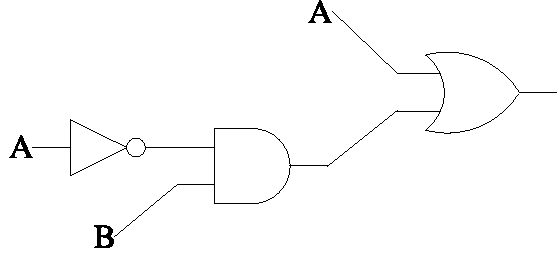
\includegraphics[width=4cm]{pictures/boole/boolt-c-ABC}
		   \end{center}}
        \alakohta{\begin{center}
		   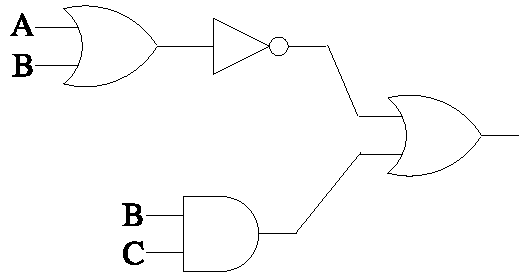
\includegraphics[width=4.5cm]{pictures/boole/boolt-d-ABC}
		   \end{center}}
    \end{alakohdat}

    \begin{vastaus}
        \begin{alakohdat}
            \alakohta{$\lnot A\lor B$}
            \alakohta{$\lnot(A\lor B)$}
            \alakohta{$A\lor (\lnot A \land B)$}
            \alakohta{$\lnot(A\lor B)\lor(B\land C)$}
        \end{alakohdat}
    \end{vastaus}
    
\end{tehtava}

\begin{tehtava}
    Piirrä lausetta
    \begin{alakohdat}
        \alakohta{$\lnot A \land B$}
        \alakohta{$A\lor \lnot (B\land C)$}
        \alakohta{$(A\land B)\lor (\lnot A \land C)$
vastaava looginen piiri.}
    \end{alakohdat}

    \begin{vastaus}
        \begin{alakohdat}
            \alakohta{KUVA!!!!!!!!!!} %Kuva puuttuu
            \alakohta{KUVA!!!!!!!!!!} %Kuva puuttuu
            \alakohta{KUVA!!!!!!!!!!} %Kuva puuttuu
        \end{alakohdat}
    \end{vastaus}
    
\end{tehtava}
%Luku 2.1 Kotitehtävät, vastausten tekijä Valtteri Vistiaho 9.11.2013
\begin{tehtava}
    Kirjoita lauseen negaatio.
    \begin{alakohdat}
        \alakohta{$100 > 101$.}
        \alakohta{Lompakossani on rahaa korkeintaan 10 euroa.}
        \alakohta{Kaikki ryhmämme opiskelijat ovat Facebookissa.}
        \alakohta{Koulussamme on täsmälleen kaksi vasenkätistä opettajaa.}
        \alakohta{En opiskele latinaa enkä kreikkaa.}
        \alakohta{Maarit pitää lumilautailusta tai käsitöistä muttei molemmista.}
    \end{alakohdat}

    \begin{vastaus}
        \begin{alakohdat}
            \alakohta{$100\leq101$}
            \alakohta{Lompakossani on rahaa enemmän kuin 10 euroa.}
            \alakohta{Kaikki ryhmämme opiskelijat eivät ole Facebookissa.}
            \alakohta{Koulussamme on enemmän tai vähemmän kuin kaksi vasenkätistä opettajaa.}
            \alakohta{Opiskelen latinaa tai kreikkaa.}
            \alakohta{Maarit pitää lumilautailusta ja käsitöistä tai Maarit ei pidä lumilautailusta eikä käsitöistä. ?????????} %En ole täysin varma vastauksesta
        \end{alakohdat}
    \end{vastaus}
    
\end{tehtava}

\begin{tehtava}
    Olkoot lauseet $A$: ''puutarhan portti on auki'', $B$: ''ruusut kukkivat'' ja $C$: ''menen puutarhaan''. Kirjoita suomen kielellä lauseet
    \begin{alakohdat}
        \alakohta{$\lnot A$,}
        \alakohta{$B\land C$,}
        \alakohta{$A\lor B$,}
        \alakohta{$\lnot B \land \lnot C$,}
        \alakohta{$\lnot(A\land B)$,}
        \alakohta{ $A \lor \lnot B$ ja}
        \alakohta{$(A \land C) \lor (\lnot B \land C)$.}
    \end{alakohdat}

    \begin{vastaus}
        \begin{alakohdat}
            \alakohta{Puutarhan portti on kiinni.}
            \alakohta{Ruusut kukkivat ja menen puutarhaan.}
            \alakohta{Puutarhan portti on auki tai ruusut kukkivat.}
            \alakohta{Ruusut eivät kuki enkä mene puutarhaan.}
            \alakohta{Ei ole totta, että puutarhan portti on auki ja ruusut kukkivat.}
            \alakohta{Puutarhan portti on auki tai ruusut eivät kuki.}
            \alakohta{Puutarhan portti on auki ja menen puutarhaan, tai ruusut eivät kuki ja menen puutarhaan.}
        \end{alakohdat}
    \end{vastaus}
    
\end{tehtava}

\begin{tehtava}
    Formalisoi lause.
    \begin{alakohdat}
        \alakohta{Kaino ei ole vanha ja Kaino on mies.}
        \alakohta{Kaino on vanha tai Kaino ei ole mies.}
        \alakohta{Kaino ei ole vanha mies. }
        \alakohta{Kaino ei ole vanha eikä hän ole mies.}
    \end{alakohdat}

    \begin{vastaus}
    Olkoot $A$: ''Kaino on vanha.'' ja $B$: ''Kaino on mies.''
        \begin{alakohdat}
            \alakohta{$\lnot A\land B$}
            \alakohta{$A\lor \lnot B$}
            \alakohta{$\lnot(A\land B)$}
            \alakohta{$\lnot A\land \lnot B$}
        \end{alakohdat}
    \end{vastaus}
    
\end{tehtava}

\begin{tehtava}
    Formalisoi lause.
    \begin{alakohdat}
        \alakohta{Amadeus kuuntelee klassista tai Klaus kuuntelee jazzia.}
        \alakohta{Amadeus ei kuuntele klassista, mutta Klaus kuuntelee jazzia.}
        \alakohta{Amadeus kuuntelee klassista, mutta Klaus ei kuuntele jazzia, tai sitten Hassinen kuuntelee progea.}
        \alakohta{Ei ole niin, että Amadeus kuuntelisi klassista, Klaus jazzia ja Hassinen progea.}
    \end{alakohdat}

    \begin{vastaus}
    Olkoot $A$: ''Amadeus kuuntelee klassista.'', $B$: ''Klaus kuuntelee jazzia.'' ja $C$: ''Hassinen kuuntelee progea.''
        \begin{alakohdat}
            \alakohta{$A\lor B$}
            \alakohta{$\lnot A\land B$}
            \alakohta{$(A\land \lnot B)\lor C$}
            \alakohta{$\lnot (A\land B\land C)$}
        \end{alakohdat}
    \end{vastaus}
    
\end{tehtava}

\begin{tehtava}
    
    \begin{alakohdat}
        \alakohta{Laadi totuustaulu lauseille $A\land \lnot A$ ja $A\lor \lnot A$.}
        \alakohta{Keksi atomilause $A$ ja ilmaise kohdan a) lauseet suomen kielellä.}
    \end{alakohdat}

    \begin{vastaus}
        \begin{alakohdat}
            \alakohta{
            \begin{center}
		    \begin{tabular}{|c|c|c|c|}\hline
		    $A$ & $\lnot A$ & $A\land \lnot A$ & $A\lor \lnot A$\\ \hline
		    $1$ & $0$ & $0$ & $1$  \\ %\hline
		    $1$ & $0$ & $0$ & $1$ \\
		    $0$ & $1$ & $0$ & $1$ \\
		    $0$ & $1$ & $0$ & $1$ \\ \hline
\end{tabular}
\end{center}}
            \alakohta{Ulkona sataa ja ulkona ei sada. \\ 
            Ulkona sataa tai ulkona ei sada.}
        \end{alakohdat}
    \end{vastaus}
    
\end{tehtava}
%Luku 2.1 kotitehtäviä, vastauksien tekijä Valtteri Vistiaho 10.11.2013
\begin{tehtava}
    Laadi totuustaulu lauseille
    \begin{alakohdat}
        \alakohta{$\lnot(A\lor B)$,}
        \alakohta{$\lnot A\land B$,}
        \alakohta{$(\lnot A\lor B)\land (A\lor \lnot B)$. \\ 
        Millä atomilauseiden $A$ ja  $B$ totuusarvojen yhdistelmillä lauseet ovat tosia?} 
    \end{alakohdat}

    \begin{vastaus}
        \begin{alakohdat}
            \alakohta{\begin{center}
		    \begin{tabular}{|c|c|c|c|}\hline
		    $A$ & $B$ & $A\lor B$ & $\lnot(A\lor B)$\\ \hline
		    $1$ & $1$ & $1$ & $0$ \\ %\hline
		    $1$ & $0$ & $0$ & $1$ \\
		    $0$ & $1$ & $1$ & $0$ \\
		    $0$ & $0$ & $1$ & $0$ \\ \hline
\end{tabular}
\end{center}
		    Lause on tosi, kun $A$ on tosi ja $B$ epätosi.}
            \alakohta{\begin{center}
		    \begin{tabular}{|c|c|c|c|}\hline
		    $A$ & $B$ & $\lnot A$ & $\lnot A\land B$ \\ \hline
		    $1$ & $1$ & $0$ & $0$  \\ %\hline
		    $1$ & $0$ & $0$ & $0$ \\
		    $0$ & $1$ & $1$ & $1$ \\
		    $0$ & $0$ & $1$ & $0$ \\ \hline
\end{tabular}
\end{center}
		    Lause on tosi, kun $A$ on epätosi ja $B$ tosi.}
            \alakohta{\begin{center}
		    \begin{tabular}{|c|c|c|c|c|c|c|}\hline
		    $A$ & $B$ & $\lnot A$ & $\lnot B$ & $(\lnot A\lor B)$ & $(A\lor \lnot B)$ & $(\lnot A\lor B)\land (A\lor \lnot B)$ \\ \hline
		    $1$ & $1$ & $0$ & $0$ & $1$ & $1$ & $1$ \\ %\hline
		    $1$ & $0$ & $0$ & $1$ & $0$ & $1$ & $0$ \\
		    $0$ & $1$ & $1$ & $0$ & $1$ & $0$ & $0$ \\
		    $0$ & $0$ & $1$ & $1$ & $1$ & $1$ & $1$ \\ \hline
\end{tabular}
\end{center}
		    Lause on tosi, kun $A$ ja $B$ ovat tosia.}
        \end{alakohdat}
    \end{vastaus}
    
\end{tehtava}

\begin{tehtava}
    
    \begin{alakohdat}
        \alakohta{Laadi totuustaulu lauseelle $A\lor (B\land C)$.}
        \alakohta{Laadi totuustaulu lauseelle $(A\lor B)\land C$.}
        \alakohta{Vertaa kohtien a) ja b) lauseiden totuusarvoja. Mitä voit päätellä?}
    \end{alakohdat}

    \begin{vastaus}
        \begin{alakohdat}
            \alakohta{
            \begin{center}
		    \begin{tabular}{|c|c|c|c|c|}\hline
		    $A$ & $B$ & $C$ & $(B\land C)$ & $A\lor (B\land C)$\\ \hline
		    $1$ & $1$ & $1$ & $1$ & $1$ \\ %\hline
		    $1$ & $1$ & $0$ & $0$ & $1$ \\
		    $1$ & $0$ & $1$ & $0$ & $1$ \\
		    $1$ & $0$ & $0$ & $0$ & $1$ \\
		    $0$ & $1$ & $1$ & $1$ & $1$ \\
		    $0$ & $0$ & $1$ & $0$ & $0$ \\
		    $0$ & $1$ & $0$ & $0$ & $0$ \\
		    $0$ & $0$ & $0$ & $0$ & $0$ \\ \hline
\end{tabular}
\end{center}}
            \alakohta{
            \begin{center}
		    \begin{tabular}{|c|c|c|c|c|}\hline
		    $A$ & $B$ & $C$ & $(A\lor B)$ & $(A\lor B)\land C$\\ \hline
		    $1$ & $1$ & $1$ & $1$ & $1$ \\ %\hline
		    $1$ & $1$ & $0$ & $1$ & $0$ \\
		    $1$ & $0$ & $1$ & $1$ & $1$ \\
		    $1$ & $0$ & $0$ & $1$ & $0$ \\
		    $0$ & $1$ & $1$ & $1$ & $1$ \\
		    $0$ & $0$ & $1$ & $0$ & $0$ \\
		    $0$ & $1$ & $0$ & $1$ & $0$ \\
		    $0$ & $0$ & $0$ & $0$ & $0$ \\ \hline
\end{tabular}
\end{center}}
            \alakohta{Sulkujen paikka on merkitsevä, ???????????????????} %En tiedä, mitä tehtävän tekijä tässä ajaa takaa.
        \end{alakohdat}
    \end{vastaus}
    
\end{tehtava}

\begin{tehtava}
    Olkoot lauseet $A$: ''$x\in [-3, 1]$'' ja $B$: ''$ x \in [-1, 5]$''. Formalisoi lause.
    \begin{alakohdat}
        \alakohta{$x\in [-3, 5]$,}
        \alakohta{$x\in [-1, 1]$,}
        \alakohta{$x\in [-3, -1[$}
        \alakohta{$x\in ]-\infty, -3[$  tai $x\in ]1, \infty[$ ja}
        \alakohta{$x\in]-\infty, -3[$  tai $x\in ]5, \infty[$.}
    \end{alakohdat}

    \begin{vastaus}
        \begin{alakohdat}
            \alakohta{$A\lor B$}
            \alakohta{$A\land B$}
            \alakohta{$A\land \lnot B$}
            \alakohta{$\lnot A$}
            \alakohta{$\lnot(A\land B$}
        \end{alakohdat}
    \end{vastaus}
    
\end{tehtava}

\begin{tehtava}
    Kolme koiranpentua, Alli, Buh ja Caesar ovat epäiltyinä isännän tohvelin repimisestä. Luotettava henkilö, joka puhuu aina totta, antaa seuraavan todistuksen: ''Ei ole totta, että Alli on syyllinen tai Buh ei ole syyllinen. Mutta kuitenkin Alli on syyllinen tai Caesar on syyllinen.'' Käytä atomilauseita $A$: ''Alli on syyllinen'', $B$: ''Buh on syyllinen'' ja $C$: ''Caesar on syyllinen'' ja formalisoi luotettavan henkilön lausunto. Muodosta sille totuustaulu ja päättele, mikä tai mitkä koiranpennuista ovat syyllisiä.

    \begin{vastaus}
            \begin{center}
		    \begin{tabular}{|c|c|c|c|c|c|c|}\hline
		    $A$ & $B$ & $C$ & $\lnot B$ & $\lnot(A\lor \lnot B)$ & $A\lor C$ & $\lnot(A\lor \lnot B)\land (A\lor C)$\\ \hline
		    $1$ & $1$ & $1$ & $0$ & $0$ & $1$ & $0$ \\ %\hline
		    $1$ & $1$ & $0$ & $0$ & $0$ & $1$ & $0$ \\
		    $1$ & $0$ & $1$ & $1$ & $0$ & $1$ & $0$ \\
		    $1$ & $0$ & $0$ & $1$ & $0$ & $1$ & $0$ \\
		    $0$ & $1$ & $1$ & $0$ & $1$ & $1$ & $1$ \\
		    $0$ & $0$ & $1$ & $1$ & $0$ & $1$ & $0$ \\
		    $0$ & $1$ & $0$ & $0$ & $1$ & $0$ & $0$ \\
		    $0$ & $0$ & $0$ & $1$ & $0$ & $0$ & $0$ \\ \hline
\end{tabular}
\end{center}
		    Buh ja Caesar ovat syyllisiä.
    \end{vastaus}
    
\end{tehtava}

\begin{tehtava}
    Tutkitaan lausetta ''Suomen kuningas ei ole viiksekäs''. Lause voidaan tulkita ainakin kahdella eri tavalla:
    \begin{alakohdat}
        \alakohta{Suomella on kuningas, joka ei ole viiksekäs.}
        \alakohta{Ei ole niin, että olisi olemassa Suomen viiksekästä kuningasta.}
    \end{alakohdat}
    Oletetaan, että Suomessa ei ole kuningasta. Onko lause tosi vai epätosi?

    \begin{vastaus}
        \begin{alakohdat}
            \alakohta{Epätosi}
            \alakohta{Tosi}
        \end{alakohdat}
    \end{vastaus}
    
\end{tehtava}

\begin{tehtava}
    Kissoilla lyhyen karvan aiheuttaa dominoiva geeni ja pitkän karvan resessiivinen geeni. Merkitään lyhyen karvan geeniä S ja pitkän karvan geeniä s. Kaikilla nisäkkäillä tiettyyn ominaisuuteen vaikuttaa geenipari, joista toinen geeni on saatu isältä ja toinen emolta. Jos kissan geeneistä ainakin toinen on S, niin se on lyhytkarvainen. Kissa on pitkäkarvainen vain siinä tapauksessa, että se on saanut geenin s molemmilta vanhemmiltaan.  Pentujen emokissa on pitkäkarvainen (ss) ja isäkissa lyhytkarvainen (SS tai Ss). Millaisia pentuja kissat voivat saada, kun isäkissan geenipari on
    \begin{alakohdat}
        \alakohta{SS}
        \alakohta{Ss?}
    \end{alakohdat}

    \begin{vastaus}
        \begin{alakohdat}
            \alakohta{Lyhytkarvaisia. (eli Ss)}
            \alakohta{Lyhyt- tai pitkäkarvaisia. (Ss tai ss)}
        \end{alakohdat}
    \end{vastaus}
\end{tehtava}